\documentclass[a0paper,portrait]{baposter}

\usepackage{wrapfig}
\usepackage{lmodern}

\usepackage[utf8]{inputenc} %unicode support
\usepackage[T1]{fontenc}
\usepackage{verbatim} % block comments
\usepackage{subcaption}
\usepackage{wrapfig} % wrapping text around figures
\usepackage{fontawesome} % twitter logo
\usepackage{setspace} % title spacing

\selectcolormodel{cmyk}

\graphicspath{{figures/}} % Directory in which figures are stored

\newcommand{\compresslist}{%
\setlength{\itemsep}{0pt}%
\setlength{\parskip}{1pt}%
\setlength{\parsep}{0pt}%
}

\newenvironment{boenumerate}
  {\begin{enumerate}\renewcommand\labelenumi{\textbf\theenumi.}}
  {\end{enumerate}}

\begin{document}

% \definecolor{darkgreen}{cmyk}{0.8,0,0.8,0.45}
% \definecolor{lightgreen}{cmyk}{0.8,0,0.8,0.25}
\definecolor{darkgreen}{cmyk}{1.0,0.85,0,0} % border
\definecolor{lightgreen}{cmyk}{1.0,0.65,0,0} % header
% reduce second value above (~0.15) for lighter blue

\begin{poster}
{
grid=false,
headerborder=open, % Adds a border around the header of content boxes
colspacing=1em, % Column spacing
bgColorOne=white, % Background color for the gradient on the left side of the poster
bgColorTwo=white, % Background color for the gradient on the right side of the poster
borderColor=darkgreen, % Border color
headerColorOne=lightgreen, % Background color for the header in the content boxes (left side)
headerColorTwo=lightgreen, % Background color for the header in the content boxes (right side)
headerFontColor=white, % Text color for the header text in the content boxes
boxColorOne=white, % Background color of the content boxes
textborder=none, %rectangle, % Format of the border around content boxes, can be: none, bars, coils, triangles, rectangle, rounded, roundedsmall, roundedright or faded
eyecatcher=false, % Set to false for ignoring the left logo in the title and move the title left
headerheight=0.11\textheight, % Height of the header
headershape=rectangle, % Specify the rounded corner in the content box headers, can be: rectangle, small-rounded, roundedright, roundedleft or rounded
headershade=plain,
headerfont=\Large\textsf, % Large, bold and sans serif font in the headers of content boxes
%textfont={\setlength{\parindent}{1.5em}}, % Uncomment for paragraph indentation
textfont=\textsf, % sans serif font
linewidth=1pt, % Width of the border lines around content boxes
columns=6 % max(span) = 6
}
{}
%
%----------------------------------------------------------------------------------------
%	TITLE AND AUTHOR NAME
%----------------------------------------------------------------------------------------
%
{
\vspace{0.3em}
\textsf %Sans Serif
{\setstretch{2.0}Recombination rate variation and linked selection in the \textit{Chlamydomonas reinhardtii} genome
}
} % Poster title
{\sf\vspace{0em}\\
Ahmed R. Hasan* and Rob W. Ness
\vspace{0.1em}\\
\small{Department of Cell and Systems Biology, University of Toronto, Toronto, ON M5S 3G5, Canada \\ Department of Biology, University of Toronto Mississauga, Mississauga, ON L5L 1C6, Canada
\vspace{0.2em}\\
\faEnvelope \hspace{0.05em} ahmed.hasan@mail.utoronto.ca | \faTwitter \hspace{0.05em} @ahmedrhasan | \faDesktop \hspace{0.05em} aays.github.io}
}
{\includegraphics[width=0.17\paperwidth]{figures/logo.pdf}}

\headerbox{Recombination rate variation in the genome}{name=introduction,column=0,row=0, span=3}{
\textsc{Recombination rate} (RR) variation is an important driver of genome evolution. Without recombination to uncouple selected alleles from their backgrounds, selection efficacy is reduced, affecting neutral polymorphism. This process of \textbf{linked selection} manifests as a loss of linked neutral variation, the extent of which is modulated by RR. Here, we investigated recombination rate variation in the facultatively sexual unicellular alga \textit{Chlamydomonas reinhardtii}, asking the questions: \\

% https://latex.org/forum/viewtopic.php?t=8033
\fcolorbox{black}[HTML]{E9F0E9}{\parbox{0.97\textwidth}{
\large{
  \begin{enumerate}\compresslist
  \item What is the extent of RR variation in the genome, and where in the genome is RR highest?
  \item How does RR variation relate to nucleotide diversity, and is there evidence for linked selection?
  \end{enumerate}
  }
}
}}

\headerbox{The landscape of recombination in \textit{C. reinhardtii}}{name=model,column=0,below=introduction,span=3}{

\textsc{Following} whole genome resequencing of \textit{C. reinhardtii} field isolates, we used \textbf{LDHelmet} [1] to estimate RR using population genomic data.

\subsection*{\textsf{Recombination varies over two orders of magnitude in the hotspot-punctuated genome}}

\begin{center}
    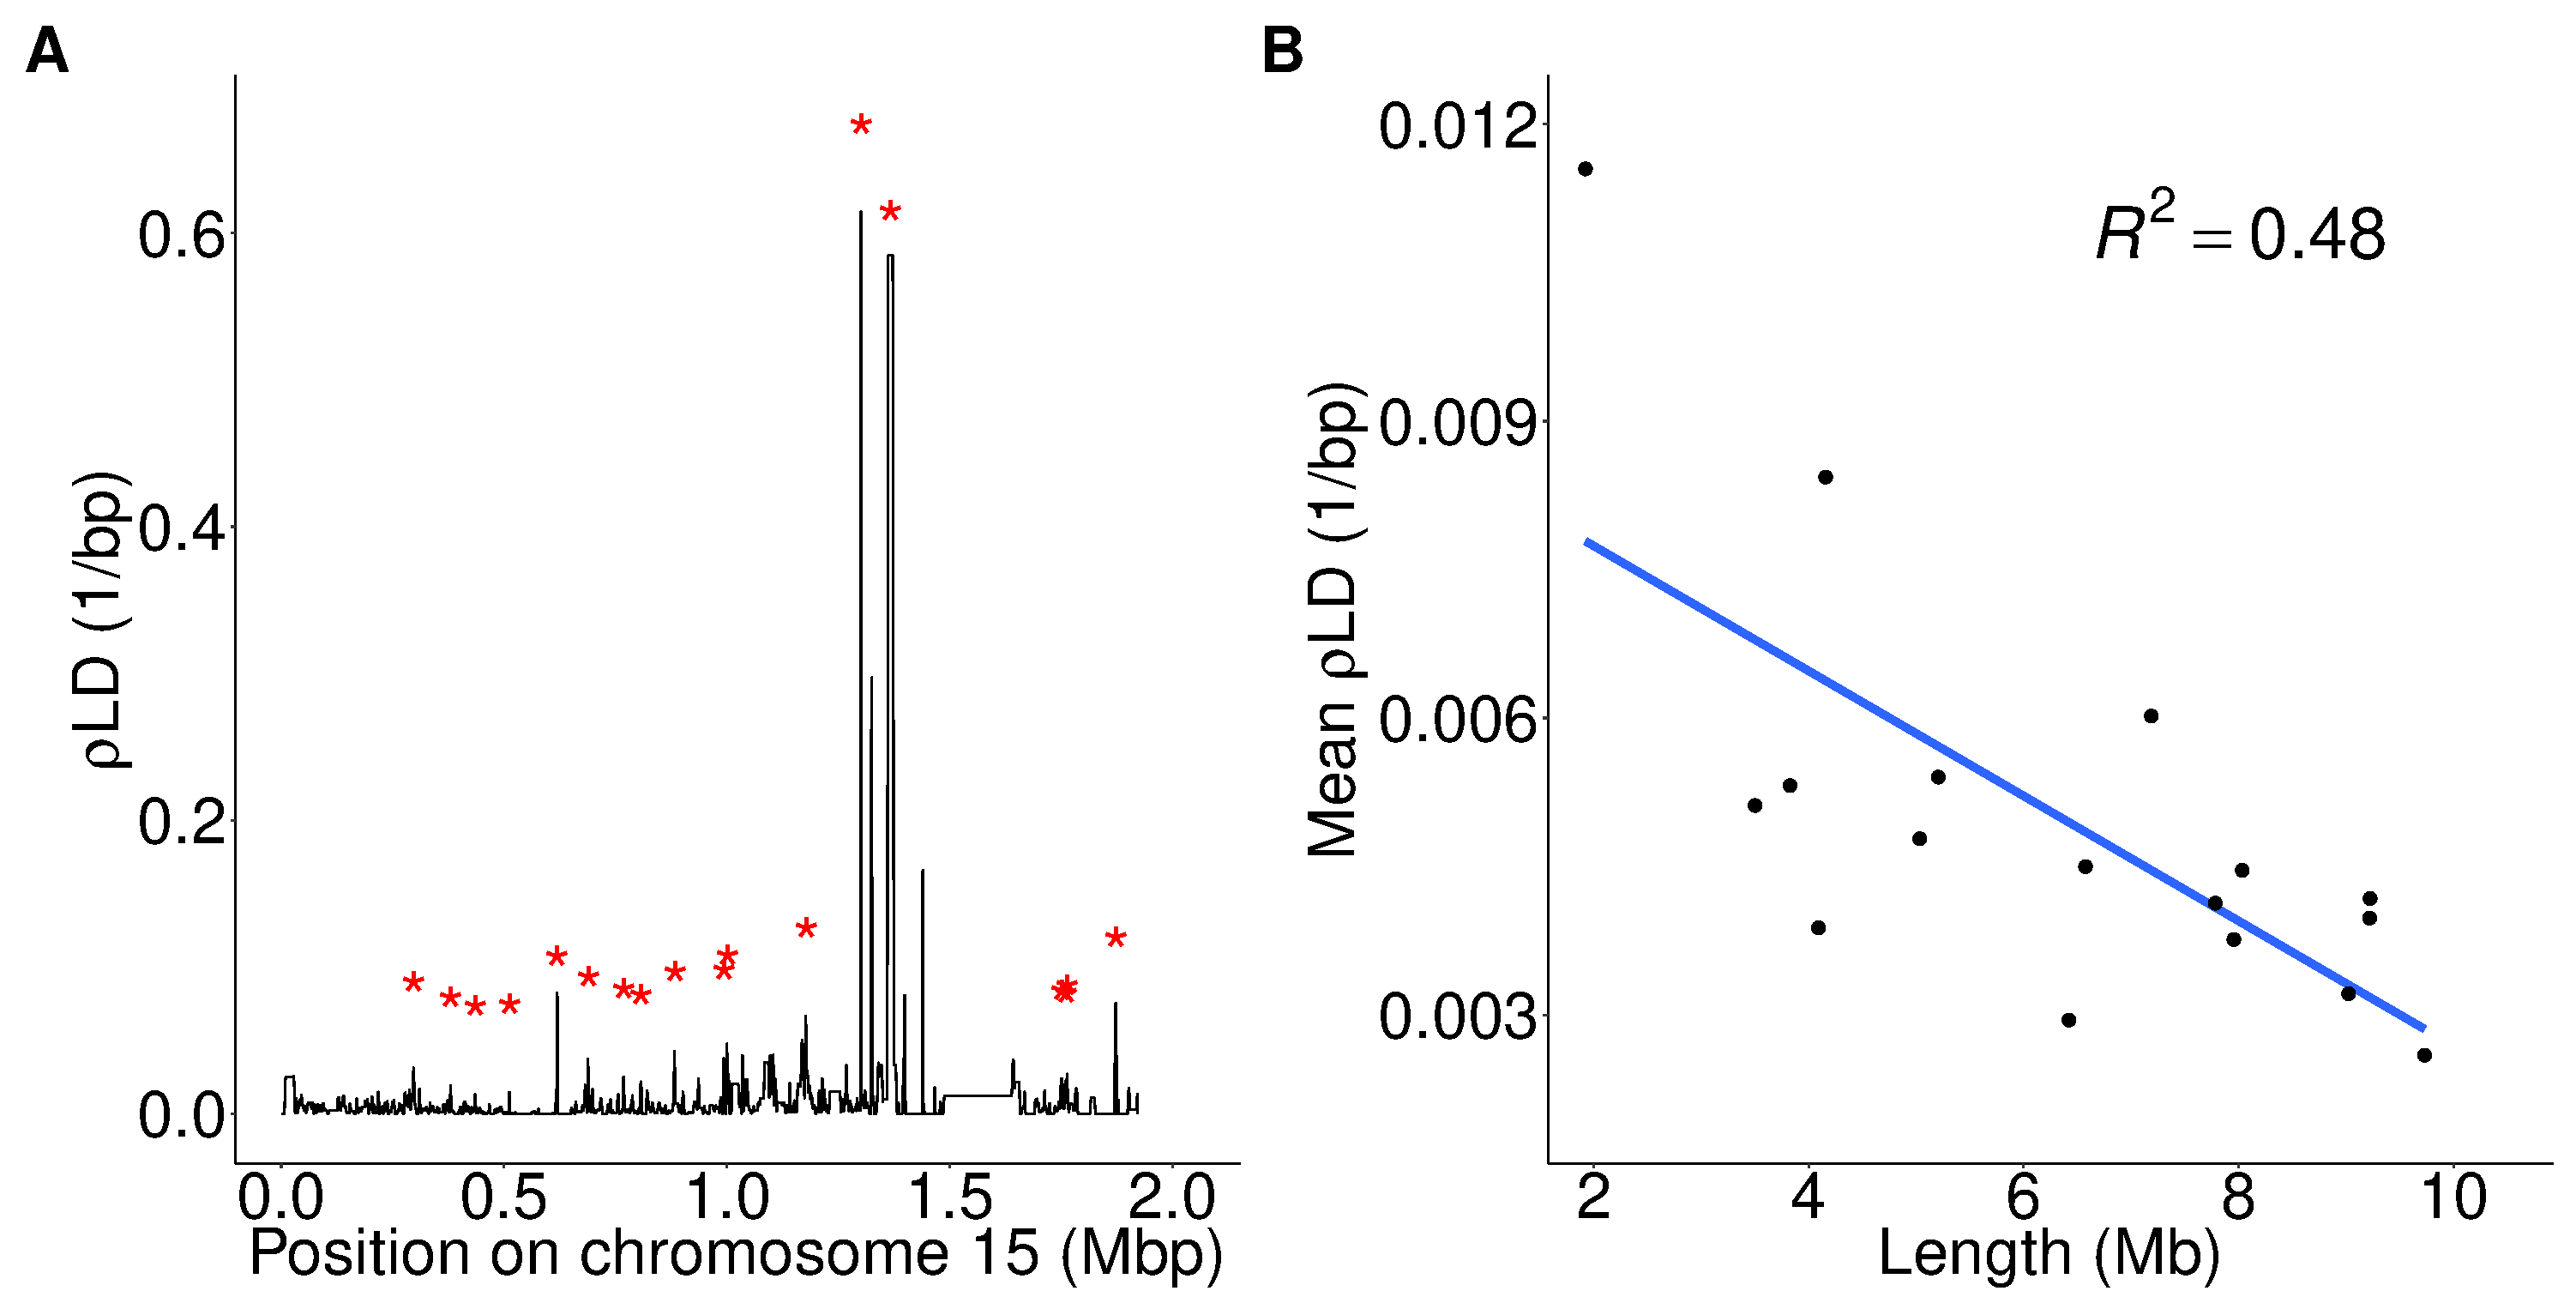
\includegraphics[width=\linewidth]{combined_fig_1_labs}
\end{center}
\textit{Fig. 1.} \textbf{A} RR variation over chromosome 15. Hotspots are indicated in red. \textbf{B} Mean chromosomal RR inversely correlates with chromosome length.

\subsection*{\textsf{Recombination rate is highest immediately flanking genes}}

\begin{center}
    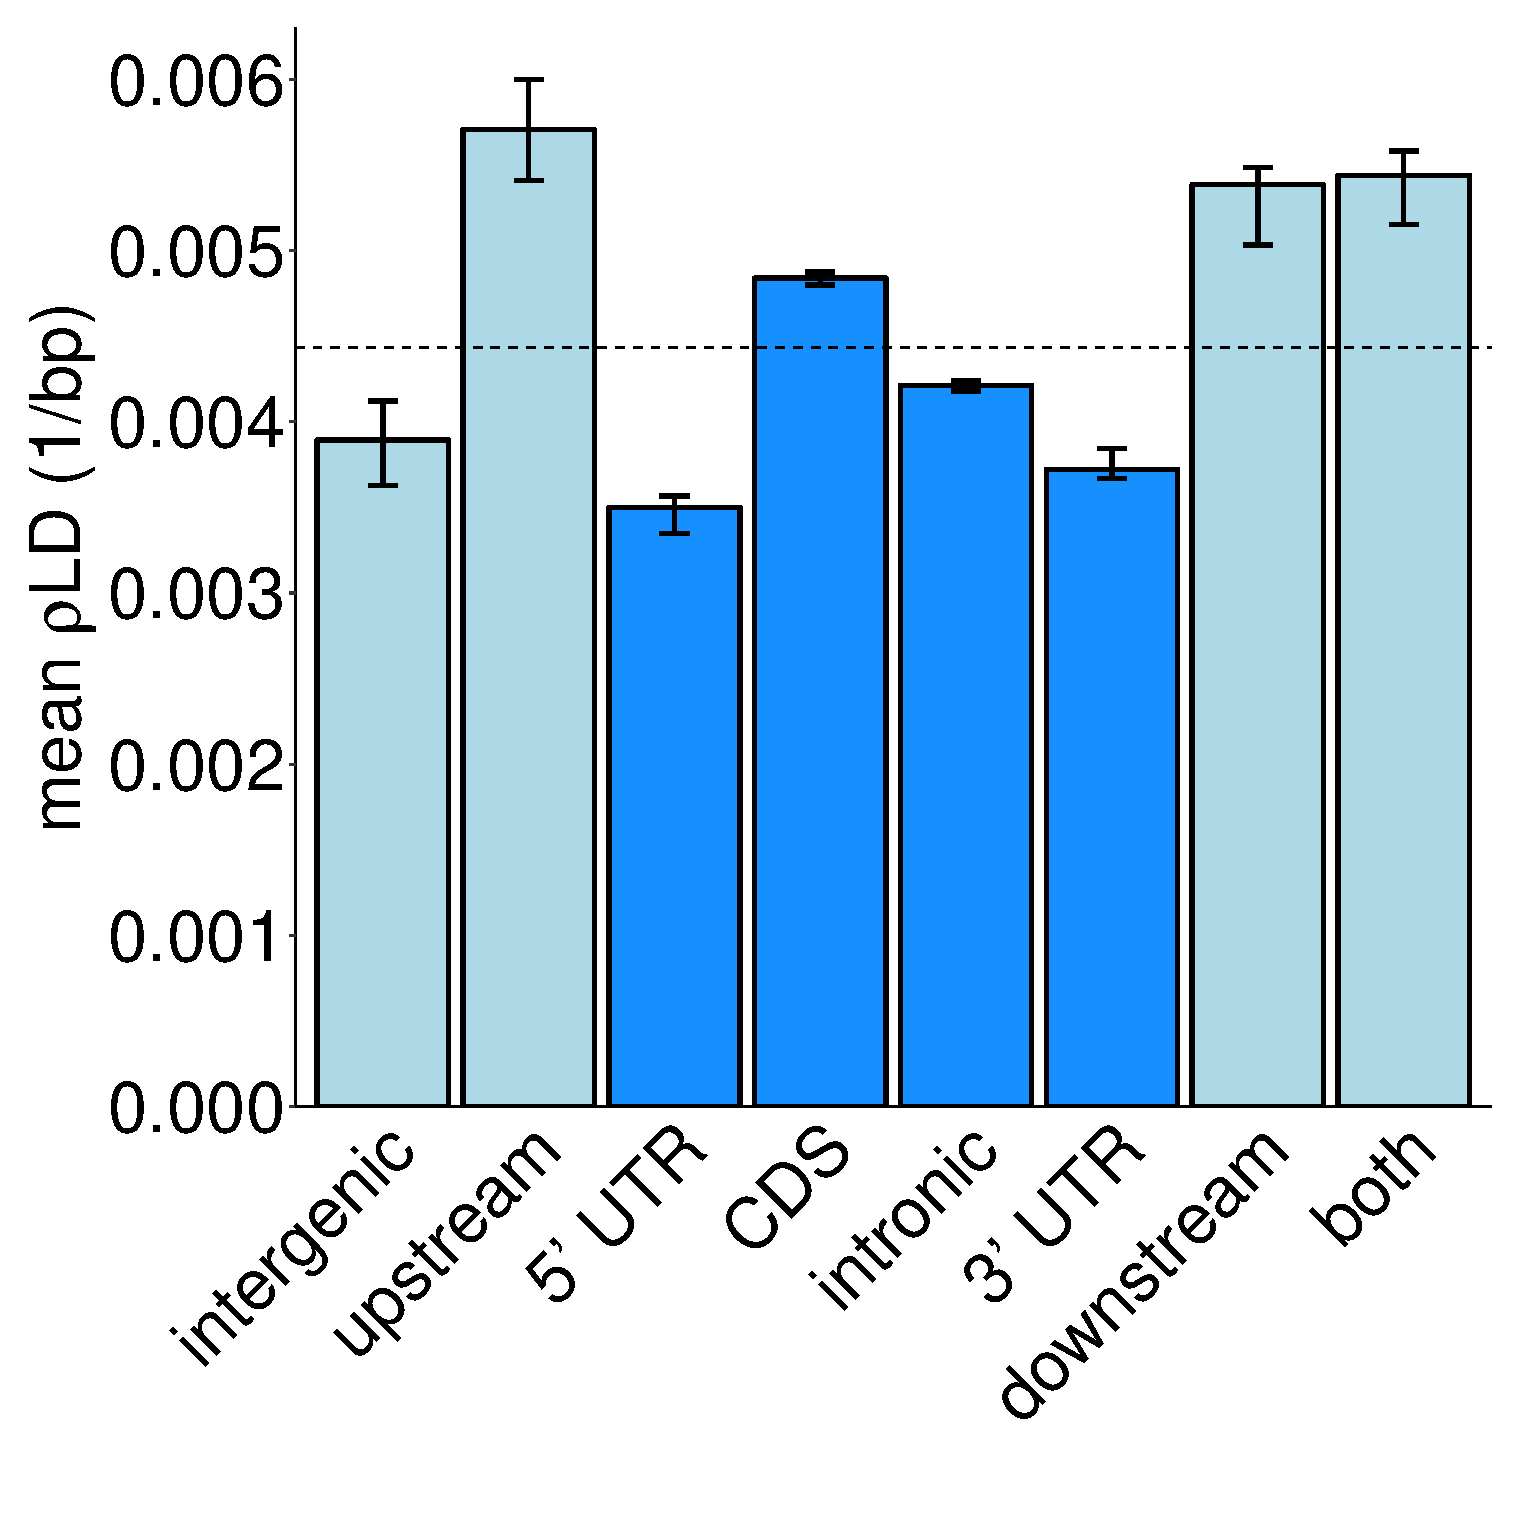
\includegraphics[width=0.6\linewidth]{correlates}
\end{center}
\textit{Fig. 2.} RR across genome annotations. RR is highest flanking genes; within genes, RR is highest in coding regions. This is consistent with patterns observed in plant recombination [2].
}

\headerbox{A role for linked selection?}{name=selection,span=3,column=3}{ 

\textsc{If} linked selection is acting in the genome, we would expect a \textbf{positive correlation between RR and neutral nucleotide diversity} ($\theta$) [3].

\subsection*{\textsf{Nucleotide diversity ($\theta_{\pi}$) correlates with LD recombination rate, but not map recombination rate}}

\begin{center}
    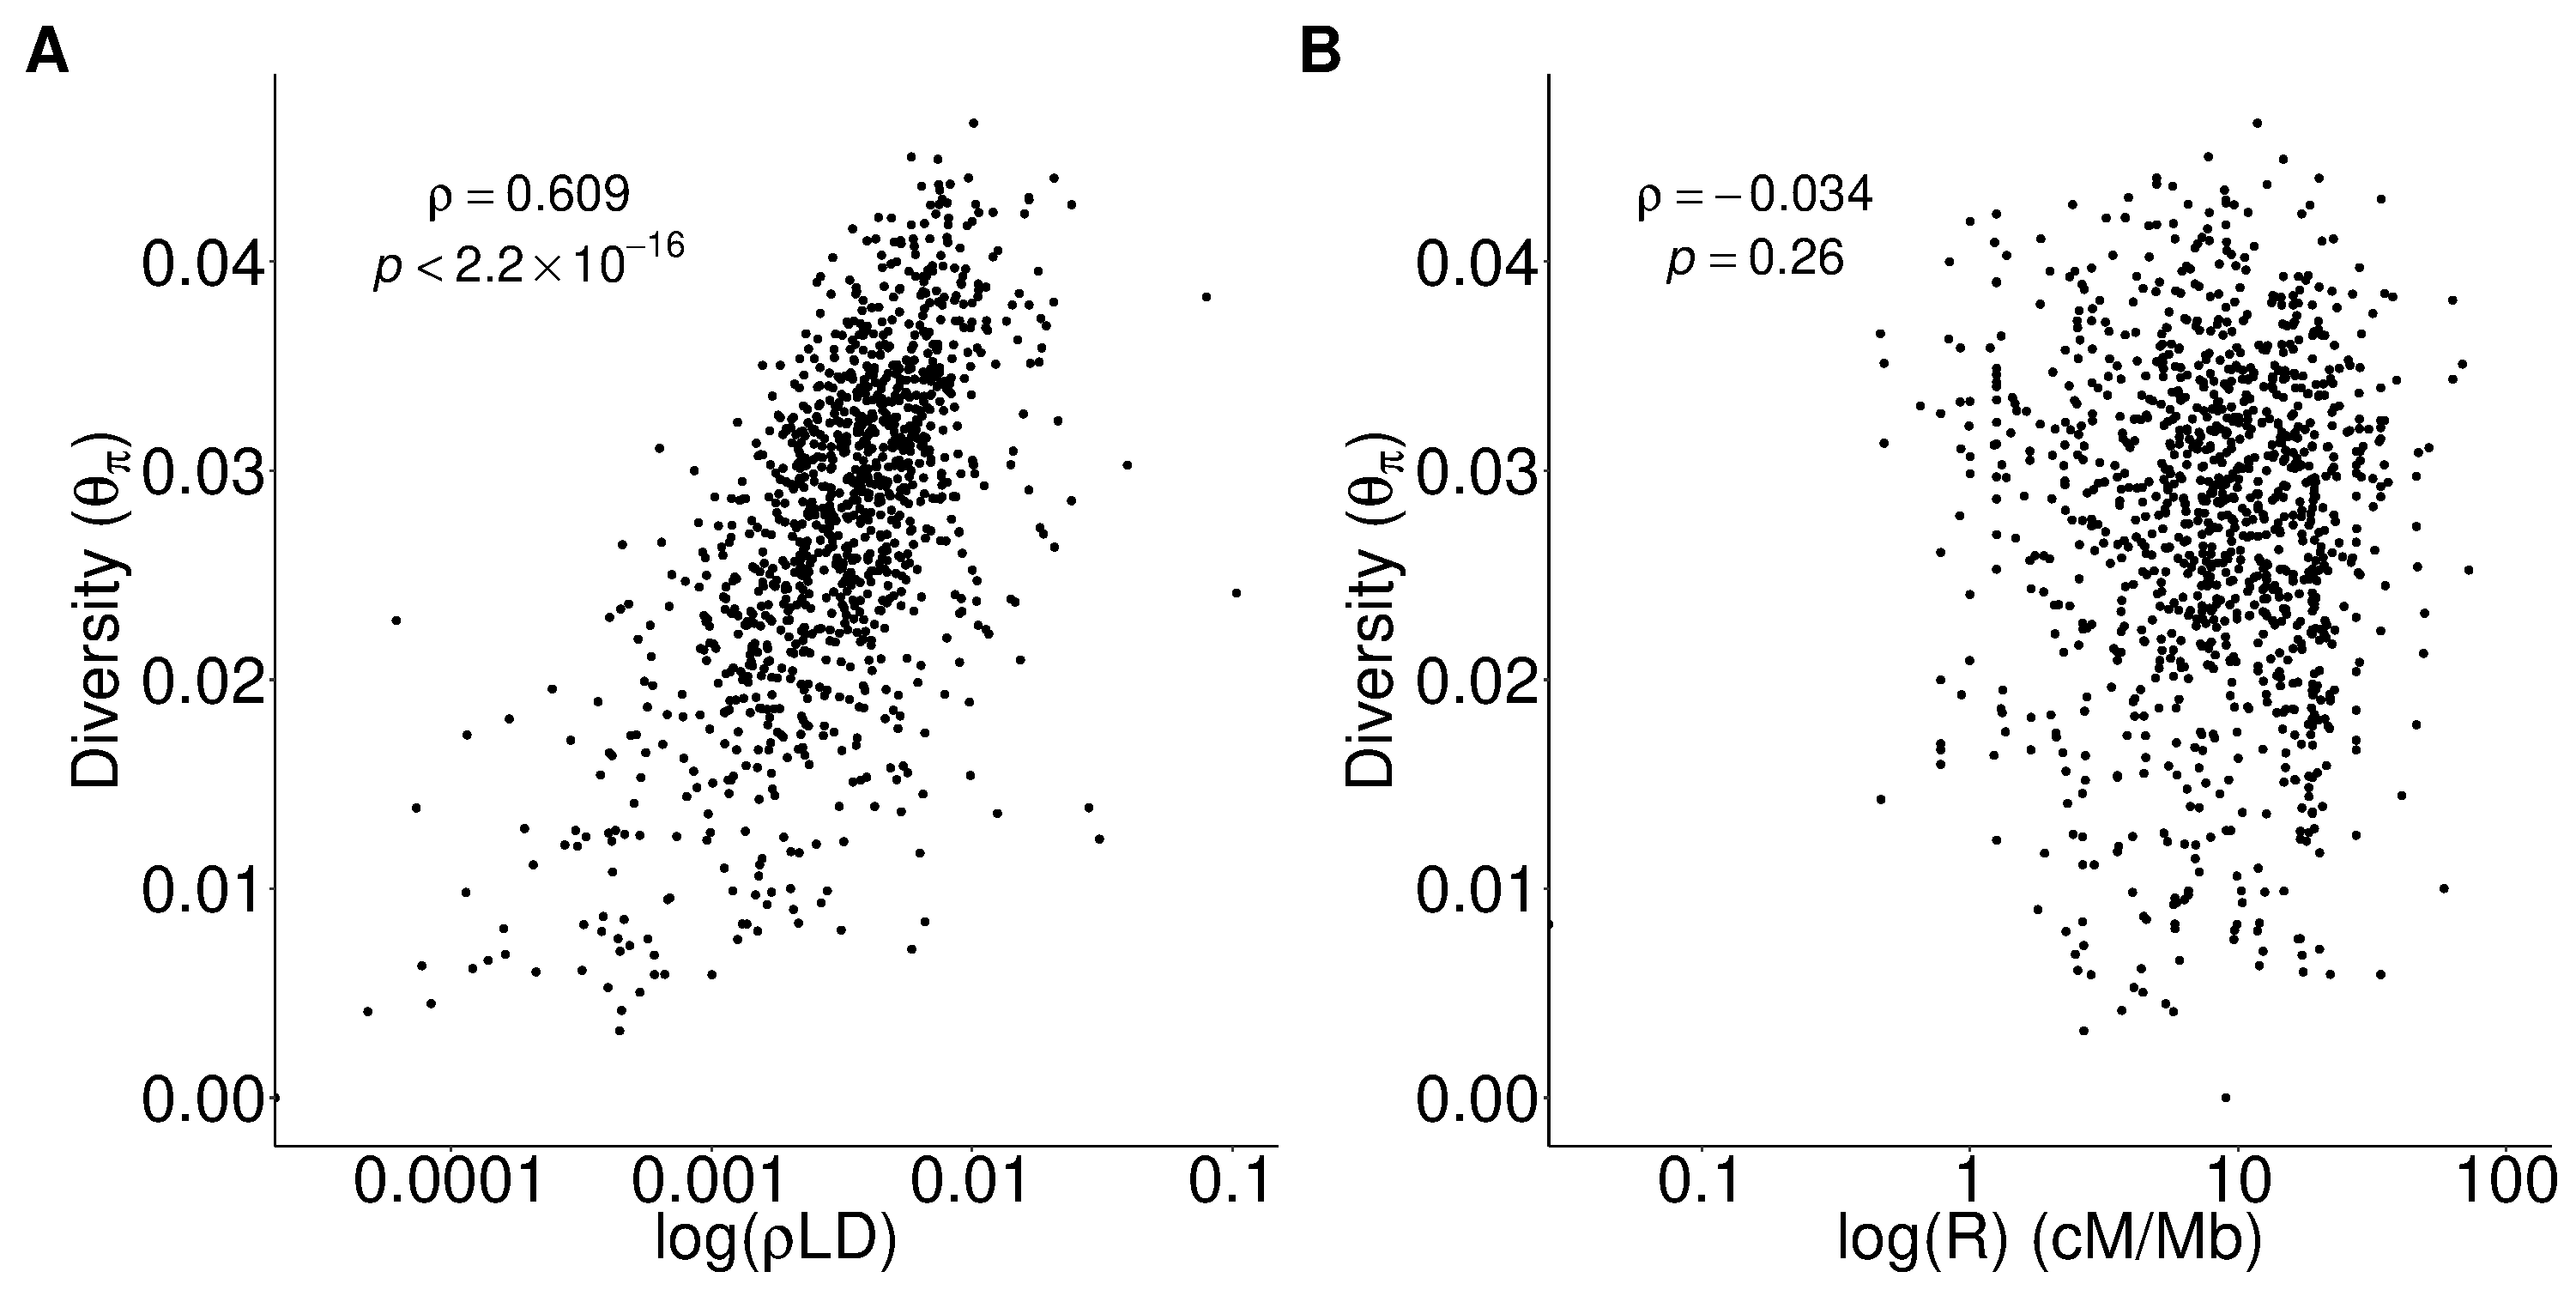
\includegraphics[width=\linewidth]{combined_fig_3_labs}
\end{center}
\textit{Fig. 3.} \textbf{A} LD recombination rate ($\rho = 4N_{e} r$) correlates with $\theta_{\pi} (=4N_{e} \mu)$. \textbf{B} Physical recombination rate estimates from the genetic map of \textit{C. reinhardtii} do not correlate with $\theta_{\pi}$. Correlations performed with Spearman's coefficient ($\rho$); values shown inline.

\subsection*{\textsf{Diversity is positively correlated with functional density}}

\textsc{The} lack of a correlation between $R$ and $\theta$ has been observed in other plant species [4,5]. In these species, diversity inversely correlates with functional density, indicating that linked selection is still acting in the genome. However, we observe the opposite pattern:

\begin{center}
    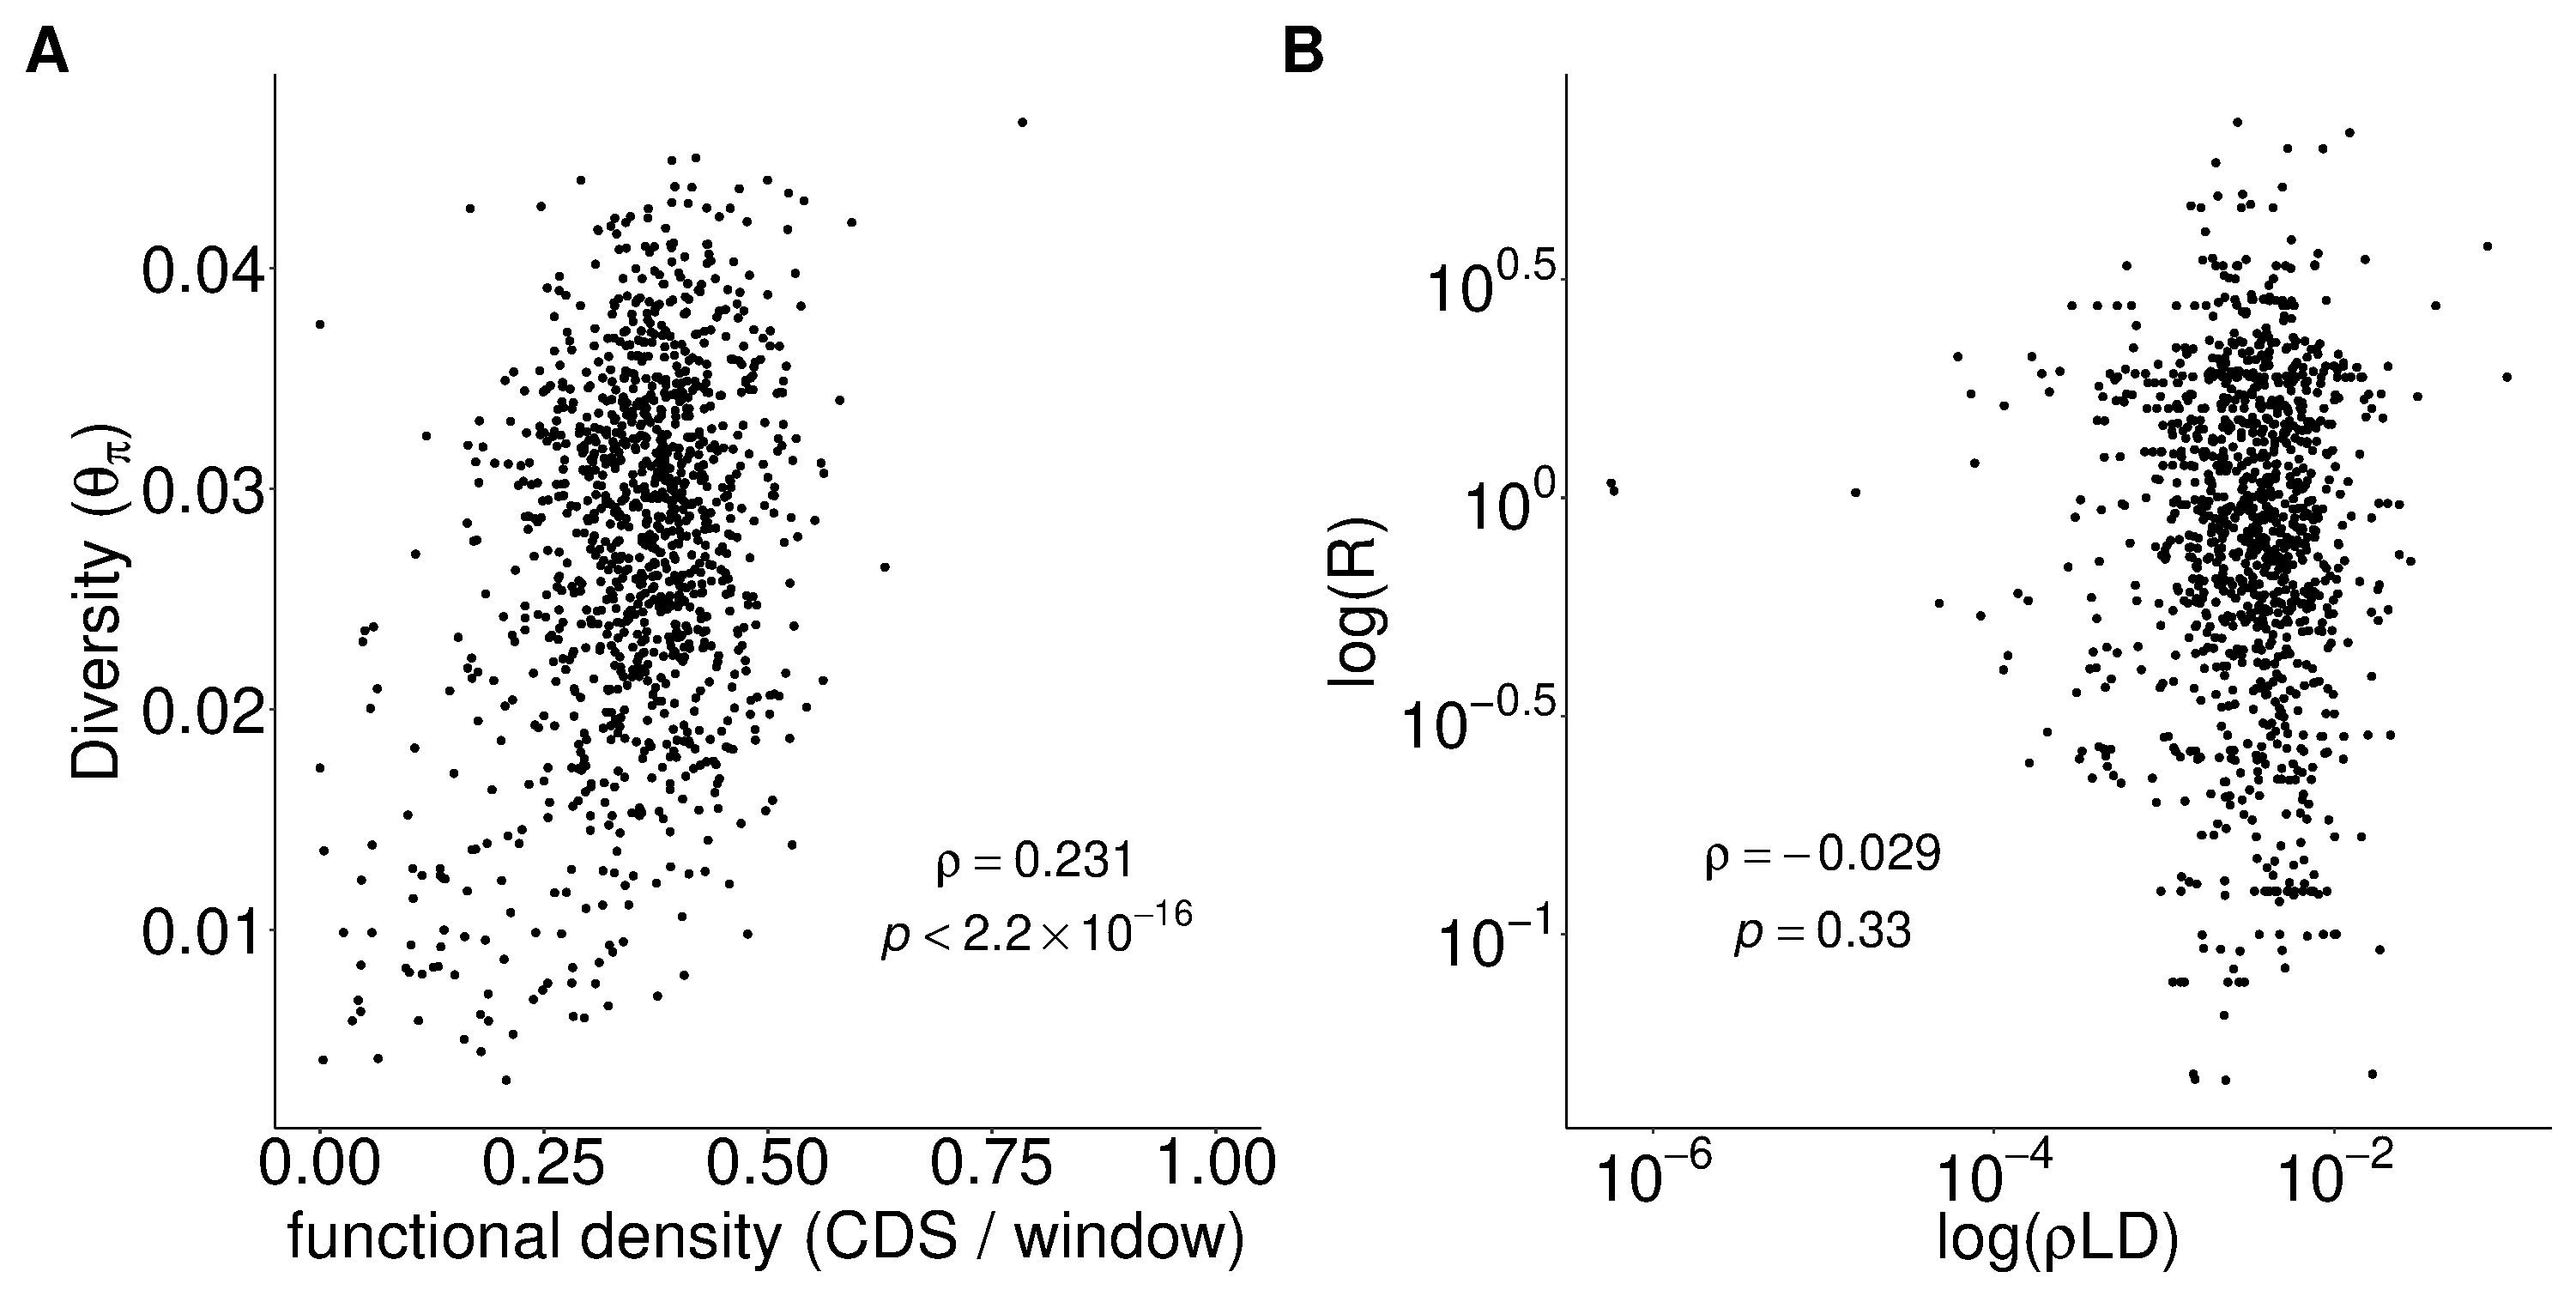
\includegraphics[width=\linewidth]{combined_fig_4_labs}
\end{center}
\textit{Fig. 4.} \textbf{A} Functional density, measured as CDS sites per 100 kb window, positively correlates with diversity. \textbf{B} LD recombination rate does not correlate with physical recombination rate. Spearman's coefficients ($\rho$) shown inline.

} % end linked selection box

\headerbox{What could be driving these patterns?}{name=conclusion,column=3,below=selection,span=3,above=bottom}{

\fcolorbox{black}[HTML]{E9F0E9}{
Why does $R$ not correlate with $\theta$ while $\rho LD$ does?
}
\begin{itemize}\compresslist
	\item Perhaps $R$ does not have enough resolution to tease apart fine-scale effects of diversity, due to insufficient marker density. We also see that $R$ does not correlate with $\rho LD$ either (Fig. 4D).
    \item $\rho LD$ and $\theta_{\pi}$ are both scaled by $N_{e}$, which may cause autocorrelation of the two variables.
\end{itemize}

\fcolorbox{black}[HTML]{E9F0E9}{
Why does diversity correlate with functional density?
}
\begin{itemize}\compresslist
	\item Not sure yet! This result is quite unexpected; population genetic theory predicts the opposite trend.
    \item A better understanding of variation in the strength of selection ($s$) across the \textit{C. reinhardtii} genome may help tease apart what factors besides recombination are playing a role. 
    \it
\end{itemize}
}


\headerbox{References}{name=references,column=0,span=3,below=model,above=bottom}{


\renewcommand{\section}[2]{\vskip 0.01em} % Get rid of the default "References" section title
\footnotesize
[1] Chan et al. \textit{PLoS Genet.,} 8(12), 2012. 
[2] Choi \& Henderson. \textit{Plant. J.} 83(1), 2015. 
[3] Begun \& Aquadro. \textit{Nature} 356, 1992.
[4] Wright et al. \textit{Genetics} 174(3), 2006.
[5] Flowers et al. \textit{Mol. Biol. Evol.} 29(2), 2012.
%\nocite{*} % Insert publications even if they are not cited in the poster


% \bibliographystyle{unsrt}
% \bibliography{poster} % Use sample.bib as the bibliography file
}

\end{poster}

\end{document}
